\documentclass[preprint, 3p,
authoryear]{elsarticle} %review=doublespace preprint=single 5p=2 column
%%% Begin My package additions %%%%%%%%%%%%%%%%%%%

\usepackage[hyphens]{url}

  \journal{MethodX} % Sets Journal name

\usepackage{lineno} % add

\usepackage{graphicx}
%%%%%%%%%%%%%%%% end my additions to header

\usepackage[T1]{fontenc}
\usepackage{lmodern}
\usepackage{amssymb,amsmath}
\usepackage{ifxetex,ifluatex}
\usepackage{fixltx2e} % provides \textsubscript
% use upquote if available, for straight quotes in verbatim environments
\IfFileExists{upquote.sty}{\usepackage{upquote}}{}
\ifnum 0\ifxetex 1\fi\ifluatex 1\fi=0 % if pdftex
  \usepackage[utf8]{inputenc}
\else % if luatex or xelatex
  \usepackage{fontspec}
  \ifxetex
    \usepackage{xltxtra,xunicode}
  \fi
  \defaultfontfeatures{Mapping=tex-text,Scale=MatchLowercase}
  \newcommand{\euro}{€}
\fi
% use microtype if available
\IfFileExists{microtype.sty}{\usepackage{microtype}}{}

\ifxetex
  \usepackage[setpagesize=false, % page size defined by xetex
              unicode=false, % unicode breaks when used with xetex
              xetex]{hyperref}
\else
  \usepackage[unicode=true]{hyperref}
\fi
\hypersetup{breaklinks=true,
            bookmarks=true,
            pdfauthor={},
            pdftitle={Optimization model for multi-product multi-period multi-supplier raw-material selection and composition, and order quantity problem with minimum one-year order quantity contract},
            colorlinks=false,
            urlcolor=blue,
            linkcolor=magenta,
            pdfborder={0 0 0}}

\setcounter{secnumdepth}{5}
% Pandoc toggle for numbering sections (defaults to be off)


% tightlist command for lists without linebreak
\providecommand{\tightlist}{%
  \setlength{\itemsep}{0pt}\setlength{\parskip}{0pt}}


% Pandoc citation processing
\newlength{\cslhangindent}
\setlength{\cslhangindent}{1.5em}
\newlength{\csllabelwidth}
\setlength{\csllabelwidth}{3em}
\newlength{\cslentryspacingunit} % times entry-spacing
\setlength{\cslentryspacingunit}{\parskip}
% for Pandoc 2.8 to 2.10.1
\newenvironment{cslreferences}%
  {}%
  {\par}
% For Pandoc 2.11+
\newenvironment{CSLReferences}[2] % #1 hanging-ident, #2 entry spacing
 {% don't indent paragraphs
  \setlength{\parindent}{0pt}
  % turn on hanging indent if param 1 is 1
  \ifodd #1
  \let\oldpar\par
  \def\par{\hangindent=\cslhangindent\oldpar}
  \fi
  % set entry spacing
  \setlength{\parskip}{#2\cslentryspacingunit}
 }%
 {}
\usepackage{calc}
\newcommand{\CSLBlock}[1]{#1\hfill\break}
\newcommand{\CSLLeftMargin}[1]{\parbox[t]{\csllabelwidth}{#1}}
\newcommand{\CSLRightInline}[1]{\parbox[t]{\linewidth - \csllabelwidth}{#1}\break}
\newcommand{\CSLIndent}[1]{\hspace{\cslhangindent}#1}

\usepackage{booktabs}
\usepackage{longtable}
\usepackage{array}
\usepackage{multirow}
\usepackage{wrapfig}
\usepackage{float}
\usepackage{colortbl}
\usepackage{pdflscape}
\usepackage{tabu}
\usepackage{threeparttable}
\usepackage{threeparttablex}
\usepackage[normalem]{ulem}
\usepackage{makecell}
\usepackage{xcolor}



\begin{document}


\begin{frontmatter}

  \title{Optimization model for multi-product multi-period
multi-supplier raw-material selection and composition, and order
quantity problem with minimum one-year order quantity contract}
    \author[a1]{Mohammad Rizka Fadhli%
  \corref{cor1}%
  }
   \ead{20921004@mahasiswa.itb.ac.id} 
    \author[a2]{Saladin Uttunggadewa%
  %
  }
   \ead{s\_uttunggadewa@math.itb.ac.id} 
    \author[a3]{Rieske Hadianti%
  %
  }
   \ead{ike.hadianti@gmail.com} 
    \author[a2]{Sri Redjeki Pudjaprasetya%
  %
  }
   \ead{srpudjap@gmail.com} 
      \affiliation[a1]{Master's Program in Computational Science;
Faculty of Mathematics and Natural Sciences; Institut Teknologi Bandung}
    \affiliation[a2]{Faculty of Mathematics and Natural Sciences;
Institut Teknologi Bandung}
    \affiliation[a3]{Center for Mathematical Modeling and Simulation;
Institut Teknologi Bandung}
    \cortext[cor1]{Corresponding author}
  
  \begin{abstract}
  This paper concerns the optimization model for a multi-product
  multi-period raw-material selection and composition, and order
  quantity problem faced by a beverage company. There are some criteria
  in raw material selection, which we accommodate all the criteria in
  the objective function. There are a number of suppliers, and one of
  the decision criteria is minimum one-year order quantity contract
  between the company and the suppliers. The actual one-year demand of
  raw materials may deviate significantly from the minimum one-year
  order quantities. In this paper, we derive a function that can be
  regarded as a penalty function in order to maintain the total order
  quantities in one year fulfil the minimum one-year order quantity
  contracts. This penalty function is a part of the objective function
  and can be relaxed once the minimum one-year order quantity contracts
  are fulfilled.

  We performed a number of numerical experiments to check the optimal
  solutions for various demands and for various objective functions.
  These experiments show our MILP gives the desired optimal solutions
  and also show the influence of decision criteria on the optimal
  solution.
  \end{abstract}
    \begin{keyword}
    inventory control \sep multi-period multi-product multi criteria
raw-material selection \sep 
    mix-integer linear programming
  \end{keyword}
  
 \end{frontmatter}

\hypertarget{introduction}{%
\section{Introduction}\label{introduction}}

This paper concerns the optimization model for supplier selection, order
allocation, and raw-material composition in a beverage company that
produces a large number of drink powders. There are a number of
suppliers that can provide the same key raw material of the drink
powders, but the color or some physical characteristics are slightly
different so we may assume those raw materials are different. The drink
powders produced by this company, which in the remainder of this paper
are called items, can be classified into two classes of items.

\begin{itemize}
\tightlist
\item
  The first class consists of items that can be produced by using
  exactly a single type of raw material.
\item
  The second class consists of more flexible items, where each item in
  this class can be produced by using one raw material or by using a
  composition of a number of raw materials. For each item in this class,
  we then have a set of possible raw materials. The sets of possible
  materials may vary from one to the other.
\end{itemize}

In order to avoid supply disruption, the company decides to use multiple
sources for these raw materials. The company has established selection
criteria for each raw material, which are based on the estimated
one-year total demand of raw materials and a subjective assessment of
whether the raw material cannot be substituted, price, service, and the
minimum order required for each purchase. After determining the score
for each raw material, the company decided to make contracts or
agreements with six suppliers. Each contract stated the unit price price
and the minimum order quantity within a year. Based on these contracts,
production planning and inventory control of raw materials are carried
out.

The estimated total one-year demand for items is obtained from the
forecasting process performed yearly. This forecasting process yields
the monthly total demand for items, which is time varying. But at the
production level, the company refines the monthly total demand on a
monthly basis as a response to some disruptions such as sudden
additional requests due to flash sales practices in e-commerce, and
others.

Once the demand for items for a month is issued, the company must
perform the decision for purchasing the raw materials from some
suppliers. This purchase decision from a supplier includes purchase for
four serial deliveries one week apart. The first delivery must be no
later than 17 days before the following month's start. The period of 17
days here is the total time required for the company's internal
inspection and preparation of raw materials.

This decision process is a complex one since there are a large number of
items that have to be produced which mostly belong to the second class,
and the monthly demand may vary. Additionally, the company imposes a
production regulation for the second class of items as a result of the
multiple-sources policy, which states that each item in the second class
must be produced using a composition of at least two types of the
corresponding possible raw materials. The decision process must be
performed carefully in order to obtain results in the form of:

\begin{itemize}
\tightlist
\item
  which raw materials are purchased along with the delivery size for
  every four corresponding weeks,
\item
  the composition of raw materials for every item in the second class
  which has to be produced,
\end{itemize}

\setlength{\parindent}{0pt} while minimizing the total inventory cost.

\setlength{\parindent}{10pt}

The company developed a decision support system for this monthly
decision process, which is developed based on an optimization model.
This paper concerns the derivation of the optimization model, which can
be categorized as a multi-product multi-period multi-supplier raw
material selection and composition, and order quantity problem. The
multi-product multi-period multi-supplier raw material selection problem
has been addressed in a number of articles such as Sambatt, Woarawichai,
and Naenna {[}1{]}, but they do not address the minimum one-year order
quantity contracts so that their optimization problem is simpler than
our optimization problem. In general, our optimization problem is much
more complex compared to the one criterion supplier selection studied in
an enormous articles such as Reck \& Long {[}2{]}, Monckza \& Trecha
{[}3{]}, \& Porter, and Harding papers. Later, supplier selection
research has developed into a problem with multiple criteria, such as
criteria for quality of goods, on time delivery, after-sales service, as
well as environmental and socio-political criteria for suppliers (see
Smytka \& Clemens {[}4{]}, Gray {[}5{]}). What is interesting is that in
general these criteria contradict each other, for example, goods offered
at low prices (positive values for the price criteria) may have negative
values for on time delivery criteria. The complexity of this issue is
compounded by the fact that some criteria are quantitative (price,
timeliness of delivery, specification/quality of goods, etc.), but other
criteria are qualitative (after-sales service, environmental and
socio-political criteria of suppliers).

The paper by Weber Current \& Benton {[}6{]} is a paper at the beginning
of this research on multi-criteria supplier selection, which presents
research results with four criteria, namely Price, Quality, Delivery and
Service (PDQS). This paper together with Hurkens, van der Valk, Wynstra
{[}7{]} introduces the supplier selection problem under the concept of
Total Cost Ownership (TCO), a financial analysis tool to examine the
direct and indirect costs of a product's production. These direct and
indirect costs then become the criteria in the supplier selection
process. These papers on TCO include Ferrin \& Plank {[}8{]}, Degraeve
\& Roodhooft {[}9{]}. Our optimization problem is categorized as a
multi-criteria one, where one of the criteria is a new one, i.e the
minimum one-year order quantity.

After the rise of conceptual research on supplier selection with
multi-criteria, then we quite easily find a proposal to use the Analytic
Hierarchy Process (AHP), a decision-making method when it comes to
ranking of many criteria (see Dyer {[}10{]}), as a method of solving
supplier problems. selection. AHP provides a framework for addressing
various criteria involving intuitive, rational, qualitative and
quantitative aspects. Other papers that discuss the AHP approach to
supplier selection solutions include Bard, Belton {[}11{]}, Bhutta \&
Huq {[}12{]}, Nydick \& Hill {[}13{]}.

Another method proposed as a solution to the supplier selection problem
is an optimization method or mathematical programming as proposed by
Degraeve \& Roodhooft {[}9{]}, Khalifa \& Mohammed Al-Shabi {[}14{]},
and Nispeling {[}15{]}. A special optimization method, namely
multi-objective goal programming, was proposed by Weber \& Ellram
{[}16{]}. Multi-objective programming is very suitable to be used to
resolve conflicts between existing criteria and the existence of
just-in-time scenarios. Meanwhile, Masella \& Rangone {[}17{]} offer a
dynamic programming method as a method of completing this supplier
selection, where input variables are set as controls and environmental
variables and status variables are set as the internal workings of the
organization, and output variables are seen as company performance.
Another optimization method used as a solution method is Data
Envelopment Analysis (DEA), as proposed in the paper of Pitchipoo, et
al. {[}18{]} and Shahrzad, et al. {[}19{]}.

Apart from these methods, we get the combined use of the two methods
above (hybrid method), such as the one proposed by Li, Wong, \& Kwong
{[}20{]} which combines the AHP method and multi-objective programming.
Another approach is the metaheuristic method proposed by Alejo-Reyes, et
al. {[}21{]}. We accommodate all criteria in one objective function, so
that our optimization model can be categorized as a mix-integer linear
programming.

This paper is written as follow. After this introduction, we describe
the production planning and inventory control in the company in Section
2. After that we derive the optimization model in Section 3. In this
section, we discuss the definition of the objective function which
expresses all criteria for decision making. Then, in Section 4 we
present the result of our numerical experimentation for obtaining the
optimal solution. We end this paper by discussing the sensitivity
analysis of the decision criteria to the optimal solution which we
present in Section 5.

\hypertarget{research-methodology}{%
\section{Research methodology}\label{research-methodology}}

\hypertarget{production-planning-and-inventory-control-for-raw-materials}{%
\subsection{Production Planning and Inventory Control for Raw
Materials}\label{production-planning-and-inventory-control-for-raw-materials}}

As mentioned above, the company deals with six raw material suppliers.
The decision process for supplier selection and order allocation is
carried out every month based on the results of demand forecasting at
the beginning of the year and production performance in the previous
month. From this demand forecasting process, the company then makes the
purchase and sales agreements with all six suppliers concerning the
one-year minimum purchase, unit price, and minimum one-month delivery.
The serial process in one calendar year can be seen in figure 1. At the
beginning of a month, the company forecasts the demand for items in the
following month.

\begin{figure}

{\centering 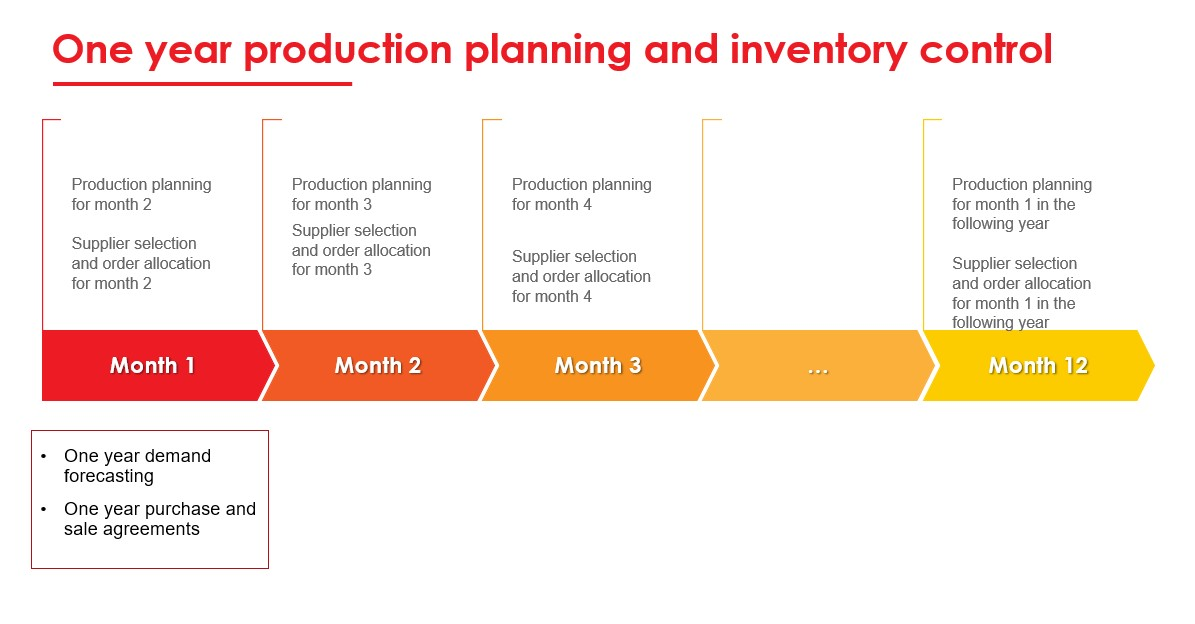
\includegraphics[width=0.8\linewidth]{production planning and inventory control} 

}

\caption{One-year production planning and inventory control}\label{fig:unnamed-chunk-1}
\end{figure}

From the estimated monthly demand for items obtained from the yearly
forecasting process, we directly can find out the estimated monthly
total demand for raw materials in one year. In practice, this one-month
estimated demand must be reviewed due to several things, such as
production in the previous month experiencing disruptions, sudden
additional requests due to flash sales practices in e-commerce, and
others. Reviewing the one-month demand and determining the production
schedule we call production planning for one month.

As soon as the production planning is performed, the company performs
the decision process for purchasing the raw materials from some
suppliers. In the following, we assume that one month can be divided
into four weeks (the fourth week may be longer than seven days). This
purchase decision covers purchases for four serial deliveries one week
apart. The first delivery must be no later than 17 days before the
following month's start since the internal inspection and the
preparation for the raw materials delivered takes 17 days. Figure 2 in
the following illustrates a one-month planning horizon and raw material
selection, and four consecutive delivery points follow it.

\begin{figure}

{\centering 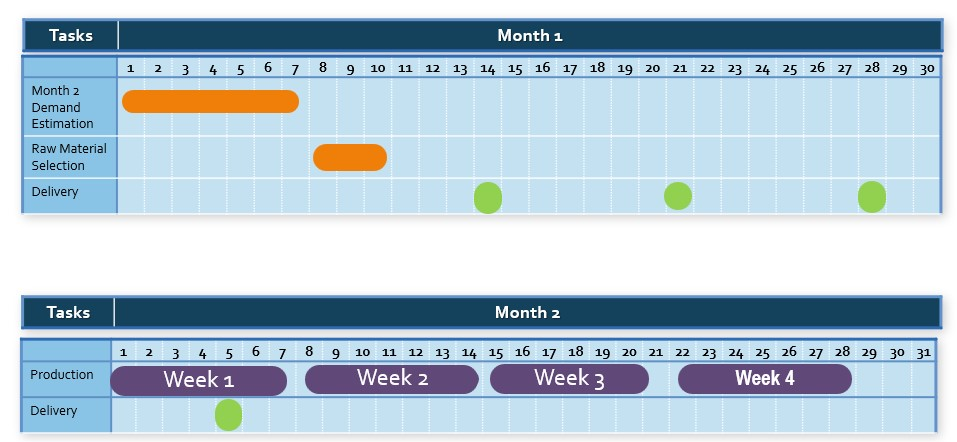
\includegraphics[width=0.8\linewidth]{Supply Cycle 2} 

}

\caption{Decision proccess planning horizon}\label{fig:unnamed-chunk-2}
\end{figure}

\newpage

The decision process considers some parameters for decision making such
as:

\begin{itemize}
\tightlist
\item
  raw materials purchase prices,
\item
  existing stock of raw materials in the warehouse,
\item
  the minimum one-month delivery of raw materials(if ordered),
\item
  the minimum one-year purchase of each raw material,
\item
  raw-material flexibility of each item, which is known by the number of
  raw materials that can be used to produce the item. The larger this
  number for an item, the more flexible the item,
\item
  and others.
\end{itemize}

The purchase must also comply with the company's internal policies in
the following.

\textbf{Policy 1.} purchase raw materials from at least two suppliers in
order to maintain supply security,

\textbf{Policy 2.} if an item must be produced by using more than one
raw material, the proportions of raw materials used are the same.

In the following section, we will accommodate all these policies into
some constraints of an optimization model that can be regarded as the
main engine of the Decision Support System developed by the company in
order to achieve an optimal decision in inventory control.

\hypertarget{mathematical-model-of-the-problem}{%
\section{Mathematical model of the
problem}\label{mathematical-model-of-the-problem}}

In this section, we formulate a mathematical model of the decision
problem. As described before, we need to make a decision for raw
material selection, delivery quantities, and raw material compositions
on the four consecutive weeks covered. In the following, we derive a
mixed integer linear programming that represent the decision problem. We
first present the sets, the parameters, and the decision variables used
in the mathematical model. We then present the constraints which
represent the production rules and capacity, followed by the discussion
concerning the objective function of the optimization model. The integer
linear programming is written after that.

\hypertarget{sets-and-parameters}{%
\subsection{Sets and parameters}\label{sets-and-parameters}}

\begin{itemize}
\tightlist
\item
  \(M = \left\{ 1,2,3,4 \right\}\) as the set of weeks on the supply
  cycle,
\item
  \(N\) as the number of raw materials,
\item
  \(\mathfrak{N}= \left\{ 1,2,...,N \right\}\) as the set of
  raw-materials,
\item
  \(I\) as the number of items,
\item
  \(\mathfrak{I} = \left\{ 1, 2, ..., I \right\}\) as the number of
  items,
\item
  \(P \bigcup_{j \in M} P_j\) as the set of items to be produced on the
  planning horizon, where \(P_j\) as the set of items to be produced on
  week \(j\).
\item
  For \(i \in \mathfrak{I}, k \in \mathfrak{N}\),
\end{itemize}

\[f_{ik} = 
\left\{\begin{matrix}
1 & , & \text{if item } i \text{ can be produce by using raw material } k  \\ 
0 & , & \text{otherwise}
\end{matrix}\right. 
\]

\begin{itemize}
\tightlist
\item
  For \(j \in M, D_j\) as the set of the total demand on week \(j\).
\item
  For \(k \in \mathfrak{N}, mo_k\) as the the one-year minimum order
  quantity of raw material \(k\).
\item
  For \(k \in \mathfrak{N}, c_k\) as the unit price of raw material
  \(k\).
\item
  For \(k \in \mathfrak{N}, \sigma_k\) as the minimum one-month order
  quantity of raw material \(k\), if purchased,
\item
  For \(k \in \mathfrak{N}, z_{0k}\) as the level of inventory of raw
  material \(k\) just before the first delivery on the first week,
\item
  \(ss\) as the safety stock for each raw material at the end of each
  week,
\item
  \(maxcap\) as the warehouse capacity,
\item
  \(hc\) as the holding cost per item per week.
\end{itemize}

\hypertarget{decision-variables}{%
\subsubsection{Decision variables}\label{decision-variables}}

Define:

\begin{itemize}
\tightlist
\item
  \(\forall k \in N, x_k\) as the amount of raw material \(k\)
  purchased. \(x_k = 0\) if raw material \(k\) is not purchased, and
  \(\sigma_k \leq x_k \leq D\) otherwise.
\item
  \(\forall k \in N\),
\end{itemize}

\[y_k = 
\left\{\begin{matrix}
0 & , & x_k  \\ 
1 & , & \sigma_k \leq x_k \leq D
\end{matrix}\right. 
\]

\begin{itemize}
\tightlist
\item
  The variables \(y_k\) are defined to handle the discontinuity property
  of the variables \(x_k\).
\item
  \(\forall j \in M, \forall k \in N, \hat{x}_{jk}\) as the amount of
  raw material \(k\) delivered at the beginning of week \(j\).
\item
  \(\forall j \in M, \forall i \in P_j, \forall k \in N,\)
\end{itemize}

\[a_{ijk} = 
\left\{\begin{matrix}
1 & , & \text{if item } i \text{ on the week }j \text{ produced by using raw material } k  \\ 
0 & , & \text{otherwise}
\end{matrix}\right. 
\]

\begin{itemize}
\tightlist
\item
  \(\forall j \in M, \forall i \in P_j, \forall k \in N, b_{ijk}\) as
  the proportion of raw material \(k\) used to produce item \(i\) on the
  week \(j\) if it uses raw material \(k\).
\item
  \(\forall j \in M, \forall k \in N, z_{jk}\) as the level of inventory
  raw material \(k\) at the end of week \(j\).
\end{itemize}

\hypertarget{constraints}{%
\subsubsection{Constraints}\label{constraints}}

The following mathematical expressions are the constraints for our
mathematical model. We write these constraints in groups where we give a
short explanation in each group the purpose of creating the constraints.

\textbf{Constraint I} are set to handle the discontinuity value of
\(x_k\). \(\forall k \in N,\)

\begin{align}
  x_k \leq y_k \space D
\end{align}

\begin{align}
  x_k \geq \sigma_k \space y_k 
\end{align}

\textbf{Constraint II} are set to fulfill the weekly allocation of each
type of raw material. \(\forall k \in N,\)

\begin{align}
  x_k = \sum_{j \in M} \hat{x}_{jk}
\end{align}

\textbf{Constraints III} are set to fulfill the raw-material demand each
week. \(\forall j \in M,\)

\begin{align}
  \sum^{N}_{k=1} \hat{x}_{jk} + \sum^{N}_{k=1} z_{(j-1)k} \geq D_j 
\end{align}

\textbf{Constraints IV} are set to ensure each item in \(P^2\) is
produced by using at least two raw materials.
\(\forall j \in M, \forall i \in P^2_j\)

\begin{align}
  \sum_{k \in N} a_{ijk} \geq 2
\end{align}

\textbf{Constraints V} concern on the relation among
\(f_{ik}, a_{ijk}, b_{ijk},\) and \(x_{jk}\).
\(\forall j \in M, i \in P, k \in N\).

\begin{align}
  a_{ijk} \leq f_{ik}
\end{align}

\(\forall j \in M, \forall i \in P, \forall k \in N\)

\begin{align}
  b_{ijk} \leq f_{ik} a_{ijk}
\end{align}

\begin{align}
  \mu a_{ijk} \leq b_{ijk}
\end{align}

for a small value of \(\mu\).

\(\forall j \in \hat{M}, \forall i \in P_j,\)

\begin{align}
  \sum_{k \in N} b_{ijk} = 1
\end{align}

\textbf{Constraints VI} are set to fulfill the Policy II.
\(\forall j \in \hat{M}, \forall i \in P^2_j, k_1, k_2 \in N, k_1 \neq k_2,\)

\begin{align}
  (1 - a_{ijk_1}) + (1 - a_{ijk_2}) \geq b_{ijk_1} - b_{ijk_2}
\end{align}

\begin{align}
  (1 - a_{ijk_1}) + (1 - a_{ijk_2}) \geq b_{ijk_2} - b_{ijk_1}
\end{align}

\textbf{Constraints VII} are set to ensure that the level of inventory
just after raw material delivery does not exceed the maximum capacity.
On the beginning of week 1,

\begin{align}
  \sum_{k \in N} (z_{0k} + \hat{x}_{1k} + z_{1k}) - D_1 \leq maxcap
\end{align}

\(\forall j \in \left\{ 2,3,4 \right\},\)

\begin{align}
  \sum_{k \in N} (z_{(j-1)k} + \hat{x}_{(j-1)k}) - \sum_{i \in P_j} b_{ijk} g_{ik} + z_jk \leq maxcap
\end{align}

\(\forall j \in M,\)

\begin{align}
  \sum_{k \in N} (z_{(j-1)k} + \hat{x}_{jk}) - \sum_{i \in P_j} b_{ijk} g_{ik} + z_jk \leq maxcap
\end{align}

\textbf{Constraints VIII} are set to ensure that the level of inventory
at the end of each week must be greater than or equal to the safety
stock. \(\forall j \in M, \forall k \in P,\)

\begin{align}
  z_{jk} \geq ss
\end{align}

\hypertarget{objective-function}{%
\subsubsection{Objective function}\label{objective-function}}

We define the objective function as the sum of the holding cost, the
purchase cost, and a function for accommodating the minimum one-year
order quantity contracts.

The level of inventory of raw-material \(k\) during one week can be seen
in figure 3.

\newpage

\begin{figure}

{\centering 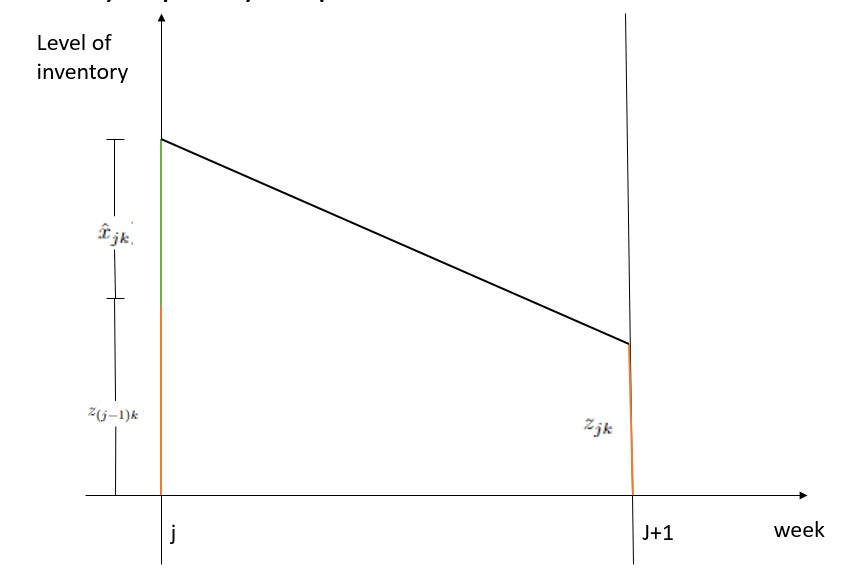
\includegraphics[width=0.7\linewidth]{inventory} 

}

\caption{Illustration for inventory cost calculation}\label{fig:unnamed-chunk-3}
\end{figure}

So that the holding cost can be given as:

\[
\frac{1}{2} hc \sum_{j \in \mathfrak{M}} \sum_{k \in \mathfrak{N}} (z_{(j-1)k} + z_{jk} + \hat{x}_{jk})
\]

Meanwhile the purchase cost can be given as:

\[
  \sum_{k \in \mathfrak{N}} c_k x_k
\]

We consider another function in the objective function, which is created
to accommodate the one-year minimum order quantity contracts.

Constraints I - VIII concern fulfillment of the minimum one-month order
quantity contract, the monthly demand, warehouse capacity constraint,
safety stock constraint, and raw material composition requirements.
Meanwhile, the one-year minimum order quantity contract is quite
difficult to be expressed as a constraint in the optimization model that
has a one-month-long planning horizon.

Therefore, we accommodate the yearly purchase contract which we
represent as a part of the objective function of our optimization
problem. To fulfill the one-year minimum order quantity contracts, we
define a penalty function:

\[
  - \sum_{k \in \mathfrak{N}} \alpha_k mo_k x_k
\]

where for \(k \in \mathfrak{N}, \alpha_k\) is multiplier constants that
will be discussed later. By denoting \(\bar{x}\) as the vector with
elements \(x_k\) and \(\hat{x}_{jk},\) and \(\bar{z}\) as the vector
with elements \(z_{jk}\) the objective function of our optimization
model is then can be written as:

\[
  F(\bar{x},\bar{z}) = \frac{1}{2} hc \sum_{j \in \mathfrak{M}} \sum_{k \in \mathfrak{N}} (z_{(j-1)k} + z_{jk} + \hat{x}_{jk}) + \sum_{k \in \mathfrak{N}} c_k x_k - \sum_{k \in \mathfrak{N}} \alpha_k mo_k x_k
\]

\hypertarget{optimization-model}{%
\subsubsection{Optimization model}\label{optimization-model}}

The optimization model for supplier selection, order allocation, and raw
material composition can be written as a mixed integer linear
programming:

\[
\begin{matrix}
\text{minimize} & F(\bar{x},\bar{z}) \\
\text{subject to} & \text{Constraint I-VIII} \\
 & x_k, \hat{x}_{jk}, z_{jk} \in \mathbb{Z}^+, y_k, a_{ijk} \in \left\{0,1 \right\}, 0 \leq b_{ijk} \leq 1
\end{matrix}
\]

where the set of \textbf{Constraints I} up to \textbf{Constraints VIII}
are given by equations (1) - (15).

\hypertarget{results}{%
\section{Results}\label{results}}

In this section, we give an example of the solution of the optimization
model we derived in the previous section. In this example, we consider
an instant where \(N=6\) and \(I=51,\) so that we have 2508 decision
variables.

\hypertarget{parameters-values}{%
\subsection{Parameters values}\label{parameters-values}}

The following tables show the matrix of raw-material flexibility of all
items.

\begin{table}[!h]

\caption{\label{tab:unnamed-chunk-4}the flexibility matrix of items 1-25}
\centering
\begin{tabular}[t]{r|r|r|r|r|r|r}
\hline
\multicolumn{1}{c|}{ } & \multicolumn{6}{c}{Raw material} \\
\cline{2-7}
item & 1 & 2 & 3 & 4 & 5 & 6\\
\hline
1 & 1 & 1 & 0 & 1 & 0 & 0\\
\hline
2 & 1 & 1 & 1 & 1 & 1 & 1\\
\hline
3 & 1 & 1 & 1 & 1 & 1 & 1\\
\hline
4 & 1 & 1 & 1 & 1 & 1 & 1\\
\hline
5 & 1 & 1 & 0 & 1 & 0 & 0\\
\hline
6 & 1 & 1 & 1 & 1 & 1 & 1\\
\hline
7 & 1 & 1 & 1 & 1 & 1 & 1\\
\hline
8 & 1 & 1 & 1 & 1 & 1 & 1\\
\hline
9 & 1 & 1 & 0 & 1 & 0 & 0\\
\hline
10 & 1 & 1 & 0 & 1 & 0 & 0\\
\hline
11 & 1 & 1 & 1 & 1 & 1 & 1\\
\hline
12 & 1 & 1 & 1 & 1 & 1 & 1\\
\hline
13 & 1 & 1 & 1 & 1 & 1 & 1\\
\hline
14 & 1 & 1 & 1 & 1 & 1 & 1\\
\hline
15 & 1 & 0 & 0 & 1 & 0 & 0\\
\hline
16 & 1 & 0 & 0 & 1 & 0 & 0\\
\hline
17 & 1 & 1 & 1 & 1 & 1 & 1\\
\hline
18 & 1 & 1 & 1 & 1 & 1 & 1\\
\hline
19 & 1 & 1 & 1 & 1 & 1 & 1\\
\hline
20 & 1 & 1 & 0 & 1 & 0 & 0\\
\hline
21 & 1 & 1 & 0 & 1 & 0 & 0\\
\hline
22 & 1 & 1 & 1 & 1 & 1 & 1\\
\hline
23 & 1 & 1 & 1 & 1 & 1 & 1\\
\hline
24 & 1 & 1 & 1 & 1 & 1 & 1\\
\hline
25 & 1 & 1 & 1 & 1 & 1 & 1\\
\hline
\end{tabular}
\end{table}
\pagebreak

\begin{table}[!h]

\caption{\label{tab:unnamed-chunk-5}the flexibility matrix of items 26-51}
\centering
\begin{tabular}[t]{r|r|r|r|r|r|r}
\hline
\multicolumn{1}{c|}{ } & \multicolumn{6}{c}{Raw material} \\
\cline{2-7}
item & 1 & 2 & 3 & 4 & 5 & 6\\
\hline
26 & 1 & 1 & 1 & 1 & 1 & 1\\
\hline
27 & 1 & 1 & 1 & 1 & 1 & 1\\
\hline
28 & 1 & 1 & 1 & 1 & 1 & 1\\
\hline
29 & 1 & 1 & 1 & 1 & 1 & 1\\
\hline
30 & 1 & 1 & 1 & 1 & 1 & 1\\
\hline
31 & 1 & 1 & 1 & 1 & 1 & 1\\
\hline
32 & 1 & 1 & 1 & 1 & 1 & 1\\
\hline
33 & 1 & 1 & 1 & 1 & 1 & 1\\
\hline
34 & 1 & 1 & 1 & 1 & 1 & 1\\
\hline
35 & 1 & 1 & 0 & 1 & 0 & 1\\
\hline
36 & 1 & 1 & 1 & 1 & 1 & 1\\
\hline
37 & 1 & 1 & 1 & 1 & 1 & 1\\
\hline
38 & 1 & 1 & 1 & 1 & 1 & 1\\
\hline
39 & 1 & 1 & 1 & 1 & 1 & 1\\
\hline
40 & 1 & 1 & 1 & 1 & 1 & 1\\
\hline
41 & 1 & 1 & 0 & 1 & 0 & 0\\
\hline
42 & 1 & 1 & 0 & 1 & 0 & 0\\
\hline
43 & 1 & 1 & 1 & 1 & 0 & 1\\
\hline
44 & 1 & 1 & 0 & 1 & 0 & 0\\
\hline
45 & 1 & 1 & 0 & 1 & 0 & 0\\
\hline
46 & 1 & 1 & 0 & 1 & 0 & 1\\
\hline
47 & 1 & 1 & 1 & 1 & 1 & 1\\
\hline
48 & 1 & 1 & 1 & 1 & 1 & 1\\
\hline
49 & 0 & 0 & 0 & 1 & 0 & 0\\
\hline
50 & 0 & 0 & 0 & 1 & 0 & 0\\
\hline
51 & 1 & 1 & 0 & 1 & 0 & 0\\
\hline
\end{tabular}
\end{table}

Next, we present the instant of the total raw material demands during a
planning horizon.

\begin{table}[!h]

\caption{\label{tab:unnamed-chunk-6}the flexibility matrix of items 1-11}
\centering
\begin{tabular}[t]{r|l|l|l|l}
\hline
\multicolumn{1}{c|}{ } & \multicolumn{4}{c}{raw -material demand (in kg)} \\
\cline{2-5}
item & week 1 & week 2 & week 3 & week 4\\
\hline
1 & 2,555.1 & 2,555.1 & 0.0 & 10,220.4\\
\hline
2 & 0.0 & 4,300.0 & 8,600.0 & 0.0\\
\hline
3 & 0.0 & 0.0 & 0.0 & 1,800.0\\
\hline
4 & 0.0 & 495.0 & 0.0 & 0.0\\
\hline
5 & 0.0 & 0.0 & 0.0 & 0.0\\
\hline
6 & 3,150.0 & 0.0 & 6,300.0 & 0.0\\
\hline
7 & 0.0 & 1,050.0 & 0.0 & 350.0\\
\hline
8 & 1,650.0 & 0.0 & 0.0 & 2,200.0\\
\hline
9 & 2,080.0 & 1,560.0 & 1,040.0 & 0.0\\
\hline
10 & 0.0 & 1,280.0 & 0.0 & 0.0\\
\hline
11 & 0.0 & 0.0 & 4,200.0 & 0.0\\
\hline
\end{tabular}
\end{table}

\newpage

\begin{table}[!h]

\caption{\label{tab:unnamed-chunk-7}the flexibility matrix of items 12-51}
\centering
\begin{tabular}[t]{r|l|l|l|l}
\hline
\multicolumn{1}{c|}{ } & \multicolumn{4}{c}{raw-material demand (in kg)} \\
\cline{2-5}
item & week 1 & week 2 & week 3 & week 4\\
\hline
12 & 0.0 & 2,700.0 & 0.0 & 0.0\\
\hline
13 & 350.0 & 350.0 & 0.0 & 0.0\\
\hline
14 & 0.0 & 300.0 & 500.0 & 200.0\\
\hline
15 & 85.0 & 0.0 & 0.0 & 0.0\\
\hline
16 & 110.0 & 165.0 & 0.0 & 0.0\\
\hline
17 & 0.0 & 0.0 & 17,400.0 & 17,400.0\\
\hline
18 & 74,050.0 & 222,150.0 & 14,800.0 & 0.0\\
\hline
19 & 0.0 & 11,605.0 & 0.0 & 0.0\\
\hline
20 & 12,750.0 & 0.0 & 0.0 & 0.0\\
\hline
21 & 3,500.0 & 0.0 & 14,000.0 & 14,000.0\\
\hline
22 & 42,100.0 & 0.0 & 10,550.0 & 0.0\\
\hline
23 & 0.0 & 0.0 & 5,600.0 & 11,200.0\\
\hline
24 & 5,400.0 & 5,400.0 & 0.0 & 5,400.0\\
\hline
25 & 1,350.0 & 2,250.0 & 0.0 & 0.0\\
\hline
26 & 0.0 & 32,400.0 & 43,200.0 & 0.0\\
\hline
27 & 10,350.0 & 31,050.0 & 0.0 & 0.0\\
\hline
28 & 118,200.0 & 0.0 & 0.0 & 0.0\\
\hline
29 & 3,330.0 & 4,995.0 & 0.0 & 0.0\\
\hline
30 & 0.0 & 1,950.0 & 0.0 & 5,850.0\\
\hline
31 & 0.0 & 6,300.0 & 6,300.0 & 0.0\\
\hline
32 & 2,310.0 & 3,465.0 & 0.0 & 0.0\\
\hline
33 & 0.0 & 2,500.0 & 0.0 & 0.0\\
\hline
34 & 0.0 & 0.0 & 20,850.0 & 0.0\\
\hline
35 & 12,150.0 & 0.0 & 0.0 & 0.0\\
\hline
36 & 0.0 & 0.0 & 0.0 & 0.0\\
\hline
37 & 12,750.0 & 12,750.0 & 8,500.0 & 8,500.0\\
\hline
38 & 1,550.0 & 3,100.0 & 0.0 & 0.0\\
\hline
39 & 0.0 & 10,600.0 & 5,300.0 & 21,200.0\\
\hline
40 & 0.0 & 0.0 & 10,450.0 & 20,900.0\\
\hline
41 & 9,625.0 & 0.0 & 1,375.0 & 1,375.0\\
\hline
42 & 0.0 & 0.0 & 3,080.0 & 0.0\\
\hline
43 & 0.0 & 2,250.0 & 450.0 & 2,250.0\\
\hline
44 & 0.0 & 0.0 & 14,100.0 & 0.0\\
\hline
45 & 6,700.0 & 13,400.0 & 10,050.0 & 6,700.0\\
\hline
46 & 6,500.0 & 13,000.0 & 0.0 & 0.0\\
\hline
47 & 26,200.0 & 13,100.0 & 0.0 & 0.0\\
\hline
48 & 12,000.0 & 8,000.0 & 0.0 & 12,000.0\\
\hline
49 & 0.0 & 126.0 & 0.0 & 0.0\\
\hline
50 & 1,323.0 & 0.0 & 3,969.0 & 0.0\\
\hline
51 & 1,170.0 & 1,170.0 & 0.0 & 780.0\\
\hline
\end{tabular}
\end{table}

We can see that items 5 and 36 do not have to be produced during this
planning horizon. We also can see that most items have to be produced
only in to or three weeks of this planning horizon, with varying demand.

The others parameters values are given in the following table.

\newpage

\begin{table}[!h]

\caption{\label{tab:unnamed-chunk-8}the other parameter's values}
\centering
\begin{tabular}[t]{ccccccc}
\toprule
\multicolumn{1}{c}{ } & \multicolumn{6}{c}{raw-material} \\
\cmidrule(l{3pt}r{3pt}){2-7}
  & 1 & 2 & 3 & 4 & 5 & 6\\
\midrule
price & 16.6 & 15.5 & 18.1 & 14.7 & 19.8 & 15.2\\
$\sigma_k$ (in kg) & 15,000.0 & 10,000.0 & 11,500.0 & 9,000.0 & 8,000.0 & 12,500.0\\
$z_{0k}$ (in kg) & 3,250.0 & 2,850.0 & 3,300.0 & 2,500.0 & 3,500.0 & 3,050.0\\
$m_{0k}$ (in kg) & 7,956,000.0 & 19,944,000.0 & 648,000.0 & 2,952,000.0 & 288,000.0 & 4,212,000.0\\
$ss$ (in kg) & 2,500.0 & 2,500.0 & 2,500.0 & 2,500.0 & 2,500.0 & 2,500.0\\
\bottomrule
\multicolumn{7}{l}{\rule{0pt}{1em}\textit{Note: }}\\
\multicolumn{7}{l}{\rule{0pt}{1em}maxcap (in kg) = 1,427,000}\\
\end{tabular}
\end{table}

From Table 2 we know that raw material 4 must be purchased since item 49
and 50 can be produced just by using raw material 4. The price of raw
material 4 is the lowest one. But the minimal one-year order quantity is
the second smallest. So that we may guess that on the optimal solution,
\(x_4\) will have a big value but is not the biggest one among others.

\hypertarget{optimal-solution}{%
\subsection{Optimal solution}\label{optimal-solution}}

We solve the optimization problem by creating computer codes using R
language (version 4) where the optimization problem formulation and the
solution technique used are referred to dplyr {[}22{]} and ompr {[}23{]}
libraries. This program runs on a computer with the Linux Ubuntu 20 LTS
operating system with an Intel i7 8 Cores processor and 16 GB RAM.

The values of \(x_k,k \in \mathfrak{N},\) are given in the second column
of Table 6 in the following. The weekly deliveries are given on columns
4 up to 6. We see that the total one-month order quantity exceeds the
minimum one-month order quantity \(\sigma_k,\) so that set of
Constraints I is satisfied.

\begin{table}[!h]

\caption{\label{tab:unnamed-chunk-9}Total order quantity and weekly deliveries}
\centering
\begin{tabular}[t]{cccccc}
\toprule
\multicolumn{2}{c}{ } & \multicolumn{4}{c}{weekly deliveries (in kg)} \\
\cmidrule(l{3pt}r{3pt}){3-6}
Raw Material & Order Qty
(in kg) & Week 1 & Week 2 & Week 3 & Week 4\\
\midrule
1 & 192,649 & 6,553 & 65,295 & 81,722 & 39,079\\
2 & 543,385 & 354,839 & 23,595 & 96,122 & 68,829\\
3 & 90,742 & 41,092 & 26,550 & 14,400 & 8,700\\
4 & 56,508 & 33,264 & 209 & 18,369 & 4,666\\
5 & 52,958 & 42,608 & 10,350 & 0 & 0\\
\addlinespace
6 & 202,853 & 70,728 & 111,075 & 0 & 21,050\\
Total & 1,139,094 & 6,553 & 65,295 & 81,722 & 39,079\\
\bottomrule
\end{tabular}
\end{table}

Besides the values \(x_k\) above, we also get
\(\hat{x}_{ijk}, a_{ijk}, b_{ijk}\) and values \(z_{jk}\) in the optimal
solution. We have checked that set of \textbf{Constraints II -- V} are
satisfied by this optimal solution. For brevity, we do not present those
values here. We just present and discuss some of them, to show that the
remaining constraints are satisfied.

Most values of \(b_{ijk}\) are \(0.5\) which mean most of items are
produced by using a composition of two raw materials. The values of
\(b_{ijk}\) may vary from one week to another wee, as illustrated in
Table 7. The composition of raw materials for item 46 in week 1is
different from the composition in week 2. Furthermore, Table 7 shows us
that the proportions of raw materials used for producing an item are the
same. We have checked this property through all for all and for all so
that we are sure that set of \textbf{Constraints VI} are satisfied.

\begin{table}[!h]

\caption{\label{tab:unnamed-chunk-10}the values of $b_{ijk}$ for $i = 45$ and $i = 46$}
\centering
\begin{tabular}[t]{cccccccc}
\toprule
\multicolumn{2}{c}{ } & \multicolumn{6}{c}{raw-material} \\
\cmidrule(l{3pt}r{3pt}){3-8}
item & week & 1 & 2 & 3 & 4 & 5 & 6\\
\midrule
45 & 1 & 0.00 & 0.50 & 0.00 & 0.50 & 0.00 & 0.00\\
45 & 2 & 0.50 & 0.50 & 0.00 & 0.00 & 0.00 & 0.00\\
45 & 3 & 0.50 & 0.50 & 0.00 & 0.00 & 0.00 & 0.00\\
45 & 4 & 0.50 & 0.50 & 0.00 & 0.00 & 0.00 & 0.00\\
46 & 1 & 0.33 & 0.33 & 0.00 & 0.33 & 0.00 & 0.00\\
\addlinespace
46 & 2 & 0.50 & 0.50 & 0.00 & 0.00 & 0.00 & 0.00\\
46 & 3 & 0.00 & 0.00 & 0.00 & 0.00 & 0.00 & 0.00\\
46 & 4 & 0.00 & 0.00 & 0.00 & 0.00 & 0.00 & 0.00\\
\bottomrule
\end{tabular}
\end{table}

The following table shows the composition of raw materials for items 49
and 50. We can see that these items are produced by using raw material
4, which confirm the flexibility matrix in Table 3.

\begin{table}[!h]

\caption{\label{tab:unnamed-chunk-11}the values of $b_{ijk}$ for $i = 49$ and $i = 50$}
\centering
\begin{tabular}[t]{cccccccc}
\toprule
\multicolumn{2}{c}{ } & \multicolumn{6}{c}{raw-material} \\
\cmidrule(l{3pt}r{3pt}){3-8}
item & week & 1 & 2 & 3 & 4 & 5 & 6\\
\midrule
49 & 1 & 0 & 0 & 0 & 0 & 0 & 0\\
49 & 2 & 0 & 0 & 0 & 1 & 0 & 0\\
49 & 3 & 0 & 0 & 0 & 0 & 0 & 0\\
49 & 4 & 0 & 0 & 0 & 0 & 0 & 0\\
50 & 1 & 0 & 0 & 0 & 1 & 0 & 0\\
\addlinespace
50 & 2 & 0 & 0 & 0 & 0 & 0 & 0\\
50 & 3 & 0 & 0 & 0 & 1 & 0 & 0\\
50 & 4 & 0 & 0 & 0 & 0 & 0 & 0\\
\bottomrule
\end{tabular}
\end{table}

The fulfillment of the safety stock constraint and the maximum capacity
constraint (set of \textbf{Constraints VII and VIII}) can be seen in the
following table.

\begin{table}[!h]

\caption{\label{tab:unnamed-chunk-12}The fulfillment of the safety stock constraint and the maximum capacity constraint (set of Constraints VII and VIII)}
\centering
\begin{tabular}[t]{ccccc}
\toprule
\multicolumn{1}{c}{ } & \multicolumn{4}{c}{end-of-week stock (in kg)} \\
\cmidrule(l{3pt}r{3pt}){2-5}
Raw material & week 1 & week 2 & week 3 & week 4\\
\midrule
1 & 2,501 & 2,501 & 2,500 & 2,500\\
2 & 181,743 & 2,501 & 2,500 & 2,500\\
3 & 2,500 & 2,500 & 2,500 & 2,500\\
4 & 2,500 & 2,501 & 2,501 & 2,500\\
5 & 2,500 & 2,500 & 2,500 & 2,500\\
\addlinespace
6 & 2,500 & 2,500 & 2,500 & 2,500\\
\bottomrule
\end{tabular}
\end{table}

\hypertarget{conclusion-and-discussion}{%
\section{Conclusion and Discussion}\label{conclusion-and-discussion}}

In this paper we present mixed-integer linear program (MILP) for
raw-material selection and composition, and order allocation problem
faced by a beverage company. We performed a number of numerical
experimentation to check the optimal solutions for various demands and
for various objective functions. From these experimentation we are sure
that our MILP gives the desired optimal solutions.

It should be noticed that the definition of the objective function which
accommodate the minimum one-year order quantity contract yields a
balancing of purchase price criteria and the minimum one-year order
quantity criteria. In the following table we represent the optimal
solutions obtained by using different objective functions. Notice that
the total raw materials purchased in all optimal solutions are the same,
i.e.~1,139,094 kg.

Table 10 The different of the optimal solutions obtained by using
different objective functions.

\begin{itemize}
\tightlist
\item
  Objective function 1:
\end{itemize}

\[
\frac{1}{2} hc \sum_{j \in M} \sum_{k \in \mathfrak{N}} (z_{(j-1)k} + z_{jk} + \hat{x}_{jk})
\]

\begin{itemize}
\tightlist
\item
  Objective function 2:
\end{itemize}

\[
\frac{1}{2} hc \sum_{j \in M} \sum_{k \in \mathfrak{N}} (z_{(j-1)k} + z_{jk} + \hat{x}_{jk}) + \sum_{k \in \mathfrak{N}} c_k x_k
\]

\begin{itemize}
\tightlist
\item
  Objective function 3:
\end{itemize}

\[
\frac{1}{2} hc \sum_{j \in M} \sum_{k \in \mathfrak{N}} (z_{(j-1)k} + z_{jk} + \hat{x}_{jk}) + \sum_{k \in \mathfrak{N}} c_k x_k - \sum_{k \in \mathfrak{N}} \alpha_k mo_k x_k
\]

\begin{table}[!h]

\caption{\label{tab:unnamed-chunk-13}Optimal solution comparison between different objective functions}
\centering
\begin{tabular}[t]{cccc}
\toprule
\multicolumn{1}{c}{ } & \multicolumn{3}{c}{Optimal solution} \\
\cmidrule(l{3pt}r{3pt}){2-4}
Raw material & obj function 1 & obj function 2 & obj function 3\\
\midrule
1 & 276,780 & 363,486 & 192,649\\
2 & 464,388 & 532,404 & 543,385\\
3 & 35,645 & 20,402 & 90,742\\
4 & 214,811 & 60,124 & 56,508\\
5 & 29,400 & 16,888 & 52,958\\
\addlinespace
6 & 118,070 & 145,791 & 202,853\\
Total & 1,139,094 & 1,139,094 & 1,139,094\\
\bottomrule
\end{tabular}
\end{table}

From Table 10 we see if we just use the purchase price in the objective
function, raw material 4 is purchased with the biggest amount. But since
in the distribution of \(mo_k\) raw material 4 has the second smallest
value, then if we consider this distribution in the objective function,
raw material 4 is purchased with a smaller amount.

The last thing to be discussed is the multiplier parameter \(\alpha_k\).
These parameters should be set as a positive number in early months of
the year, when the minimum one-year order quantity contracts are still
far away to be fulfilled. As soon as the contract for raw material \(k\)
is fulfilled, we can set \(\alpha_{k=0}\).

\hypertarget{acknowledment}{%
\section{Acknowledment}\label{acknowledment}}

The research in this paper is partially funded by the Penelitian Tesis
Magister research grant, Ministry of Research and Technology of the
Republic of Indonesia.

\hypertarget{references}{%
\section*{References}\label{references}}
\addcontentsline{toc}{section}{References}

\hypertarget{refs}{}
\begin{CSLReferences}{0}{0}
\leavevmode\vadjust pre{\hypertarget{ref-a1}{}}%
\CSLLeftMargin{1. }%
\CSLRightInline{Sambatt, M., Woarawichai, C., \& Naenna, T. (2018).
Inventory lot sizing and supplier selection for multiple
products,multiple suppliers, multiple periods with storage space using
lingo program. \emph{MATEC Web of Conferences 259, 04004 (2019), 2018
6th International Conference on Traffic and Logistic Engineering (ICTLE
2018)}.
https://doi.org/\url{https://doi.org/10.1051/matecconf/201925904004}}

\leavevmode\vadjust pre{\hypertarget{ref-a2}{}}%
\CSLLeftMargin{2. }%
\CSLRightInline{Reck, R. F., \& Long, B. G. (1988). Purchasing: A
competitive weapon. \emph{Journal of Purchasing and Materials
Management}, \emph{24(3)}, 2--8.}

\leavevmode\vadjust pre{\hypertarget{ref-a3}{}}%
\CSLLeftMargin{3. }%
\CSLRightInline{Monckza, R. M., \& Trecha, S. J. (1988). Cost-based
supplier performance evaluation. \emph{Journal of Purchasing and
Materials Management}, \emph{24 (1)}, 2--7.}

\leavevmode\vadjust pre{\hypertarget{ref-a4}{}}%
\CSLLeftMargin{4. }%
\CSLRightInline{Smytka, D. L., \& Clemens, M. W. (1993). Total cost
supplier selection model: A case study. \emph{International Journal of
Purchasing and Materials Management}, \emph{Volume 29, Issue 4},
42--49.}

\leavevmode\vadjust pre{\hypertarget{ref-a5}{}}%
\CSLLeftMargin{5. }%
\CSLRightInline{Gray, J. V., Helper, S., \& Osborn, B. (2020). Value
first, cost later: Total value contribution as a new approach to
sourcing decisions. \emph{Journal of Operations Management},
\emph{Volume 66, Issue 6}, 735--750.}

\leavevmode\vadjust pre{\hypertarget{ref-a6}{}}%
\CSLLeftMargin{6. }%
\CSLRightInline{Weber, C. A., Current, J. R., \& Benton, W. C. (1991).
Vendor selection criteria and methods. \emph{European Journal of
Operational Research}, \emph{50}, 2--18.}

\leavevmode\vadjust pre{\hypertarget{ref-a7}{}}%
\CSLLeftMargin{7. }%
\CSLRightInline{Hurkens, K., Valk, W. van der, \& F. Wynstra. (1993).
Total cost of ownership in the services sector: A case study.
\emph{Journal of Supply Chain Management}, \emph{Volume 29, Issue 3},
2--11.}

\leavevmode\vadjust pre{\hypertarget{ref-a8}{}}%
\CSLLeftMargin{8. }%
\CSLRightInline{Ferrin, B. G., \& Plank, R. E. (2002). Total cost of
ownership models: An exploratory study. \emph{Journal of Supply
Management}, \emph{Volume 8, Issue 2}, 18--29.}

\leavevmode\vadjust pre{\hypertarget{ref-a9}{}}%
\CSLLeftMargin{9. }%
\CSLRightInline{Degraeve, Z., \& Roodhooft, F. (2000). A mathematical
programming approach for procurement using activity based costing.
\emph{Journal of Business Finance and Accounting}, \emph{27 (1 - 2)},
69--98.}

\leavevmode\vadjust pre{\hypertarget{ref-a10}{}}%
\CSLLeftMargin{10. }%
\CSLRightInline{Dyer, J. S. (1990). Remarks on the analytic hierarchy
process. \emph{Management Science}, \emph{36}, 249--258.}

\leavevmode\vadjust pre{\hypertarget{ref-a11}{}}%
\CSLLeftMargin{11. }%
\CSLRightInline{Belton, V. (1986). A comparison of the analytic
hierarchy process and simple multi-attribute value function.
\emph{European Journal of Operational Research}, \emph{26}, 7--21.}

\leavevmode\vadjust pre{\hypertarget{ref-a12}{}}%
\CSLLeftMargin{12. }%
\CSLRightInline{Bhutta, K. S., \& Huq, F. (2002). Supplier selection
problem: A comparison of the total cost of ownership and analytic
hierarchy process. \emph{Supply Chain Management: An International
Journal}, \emph{Volume 17 (3)}.}

\leavevmode\vadjust pre{\hypertarget{ref-a13}{}}%
\CSLLeftMargin{13. }%
\CSLRightInline{Nydick, R. L., \& Hill, R. P. (1992). Using the analytic
hierarchy process to structure the supplier selection procedure.
\emph{International Journal of Purchasing and Materials Management},
\emph{Volume 28, Issue2}, 31--36.}

\leavevmode\vadjust pre{\hypertarget{ref-a14}{}}%
\CSLLeftMargin{14. }%
\CSLRightInline{Khalifa, H. A. E. W., \& Al-Shabi, M. A. (2018). Solving
the inexact rough intervals vendor selection problems. \emph{European
Journal of Scientific Research}, \emph{Volume 150 (3)}, 265--272.}

\leavevmode\vadjust pre{\hypertarget{ref-a15}{}}%
\CSLLeftMargin{15. }%
\CSLRightInline{Nispeling, T. (2015). Multi-criteria supplier selection
in the edible oil industry: The case of a new oils \& fats plant in
china. \emph{Master Thesis, TU Delf, the Netherlands}.}

\leavevmode\vadjust pre{\hypertarget{ref-a16}{}}%
\CSLLeftMargin{16. }%
\CSLRightInline{Weber, C. A., \& Ellram, L. M. (1993). Supplier
selection using multi-objective programming: A decision support system
approach. \emph{International Journal of Physical Distribution \&
Logistics Management}, \emph{23 (3)}, 3--14.}

\leavevmode\vadjust pre{\hypertarget{ref-a17}{}}%
\CSLLeftMargin{17. }%
\CSLRightInline{Masella, C., \& Rangone, A. (2000). A contingent
approach to the design of vendor selection systems for different types
of co-operative customer/supplier relationships. \emph{International
Journal of Operations \& Production Management}, \emph{Volume 20 (1)},
70--84.}

\leavevmode\vadjust pre{\hypertarget{ref-a18}{}}%
\CSLLeftMargin{18. }%
\CSLRightInline{Pitchipoo, P., Ragavan, R., Venkumar, P., \&
Sivaprakasam, R. (2013). Development of DEA decision model for supplier
selection. \emph{Proceeding of IEEE -- International Conference on
Research and Development Prospects on Engineering and Technology},
\emph{EGS Pillay Engineering College, Nagapattinam, India}.}

\leavevmode\vadjust pre{\hypertarget{ref-a19}{}}%
\CSLLeftMargin{19. }%
\CSLRightInline{Shahrzad, T., Mohammad, E., \& Reza, R. S. M. (2021).
Integration of DEA (data envelopment analysis) approach for supplier
selection with hierarchical analysis process and risk considerations.
\emph{presented at INTERNATIONAL CONFERENCE ON MANAGEMENT, TOURISM AND
TECHNOLOGY, Malaysia, November 2021}.}

\leavevmode\vadjust pre{\hypertarget{ref-a20}{}}%
\CSLLeftMargin{20. }%
\CSLRightInline{Li, Z., Wong, W. K., \& Kwong, C. K. (2013). An
integrated model of material supplier selection and order allocation
using fuzzy extended AHP and multi-objective programming.
\emph{Mathematical Problems in Engineering}, \emph{Volume 2013, Article
ID 362718, Hindawi Publishing Corporation}.}

\leavevmode\vadjust pre{\hypertarget{ref-a21}{}}%
\CSLLeftMargin{21. }%
\CSLRightInline{Alejo-Reyes, A., Cuevas, E., Rodriguez, A., Mendoza, A.,
\& Olivares-Benitez, E. (2020). An improved grey-wolf optimizer for a
supplier selection and order quantity allocation problem.
\emph{Mathematics}, \emph{8 (9)}.}

\leavevmode\vadjust pre{\hypertarget{ref-dplyr}{}}%
\CSLLeftMargin{22. }%
\CSLRightInline{Wickham, H., François, R., Henry, L., Müller, K., \&
Vaughan, D. (2023). \emph{Dplyr: A grammar of data manipulation}.}

\leavevmode\vadjust pre{\hypertarget{ref-ompr}{}}%
\CSLLeftMargin{23. }%
\CSLRightInline{Schumacher, D. (2022). \emph{Ompr: Model and solve mixed
integer linear programs}. Retrieved from
\url{https://github.com/dirkschumacher/ompr}}

\end{CSLReferences}


\end{document}
